\section{Resultados}

A lo largo de esta sección se presentan los resultados de los procedimientos descritos en la metodología. 

\subsection{Análisis de la Red}

\subsection{Optimización de Hiperparámetros}

El proceso de optimización de hiperparámetros mediante el BHO se analizará mostrando el frente de pareto de ambos algoritmos y una visualización del rendimiento marginal de ambas métricas en base al valor de resolución (\(\gamma\)) evaluado.

\begin{figure}[htbp]
	\centering
	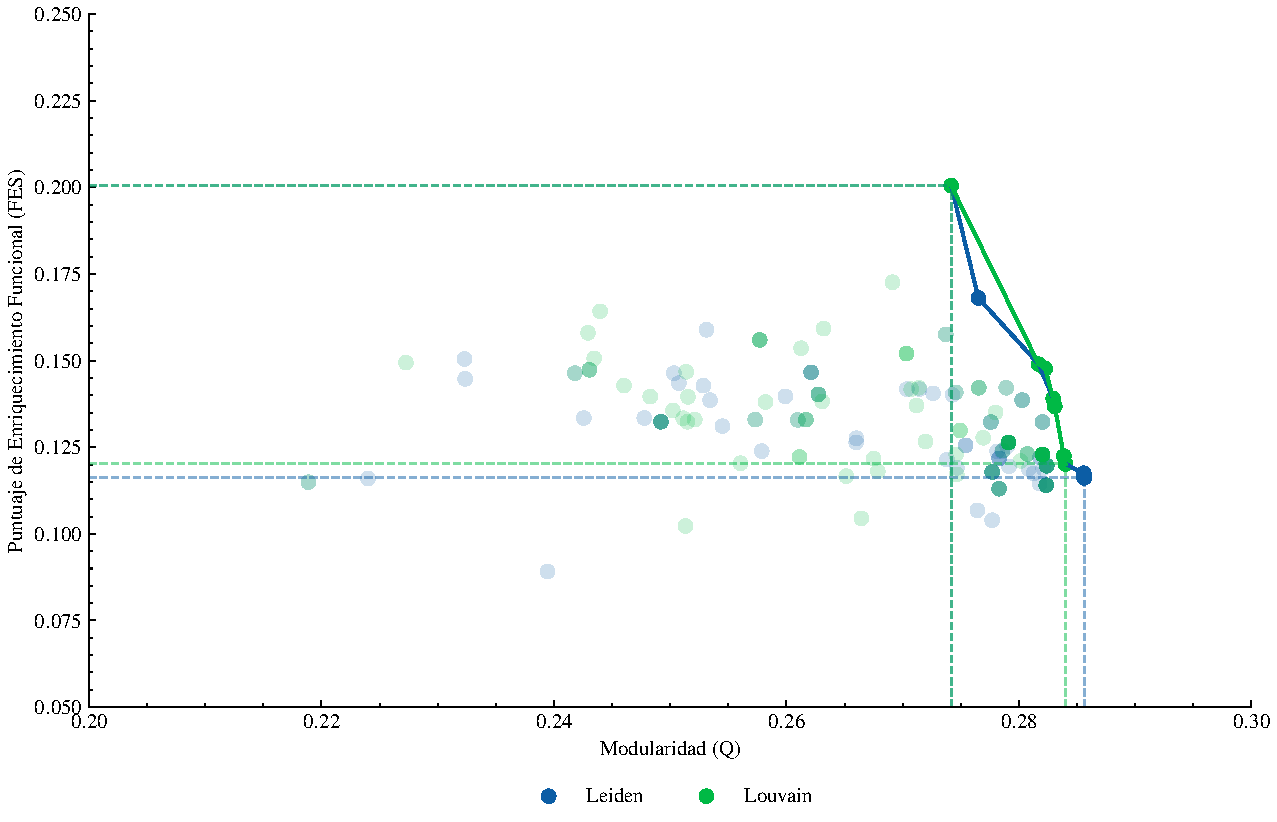
\includegraphics[width=.96\textwidth]{../results/plots/optimization/pareto_comparison.pdf}
	\caption{Frente de Pareto obtenido tras maximizar el puntuaje de FES y el coeficiente Q para Leiden y Louvain. Se puede observar que, para las soluciones Pareto-eficientes que conforman el extremo de la frontera, Leiden obtiene un puntuaje superior en cuanto a la modularidad, mientras que ambos algoritmos están igualados en cuanto al puntuaje de enriquecimiento funcional, diferenciándose por pocos decimales.}
	\label{fig:pareto}
\end{figure}

\begin{figure}[htbp]
	\centering
	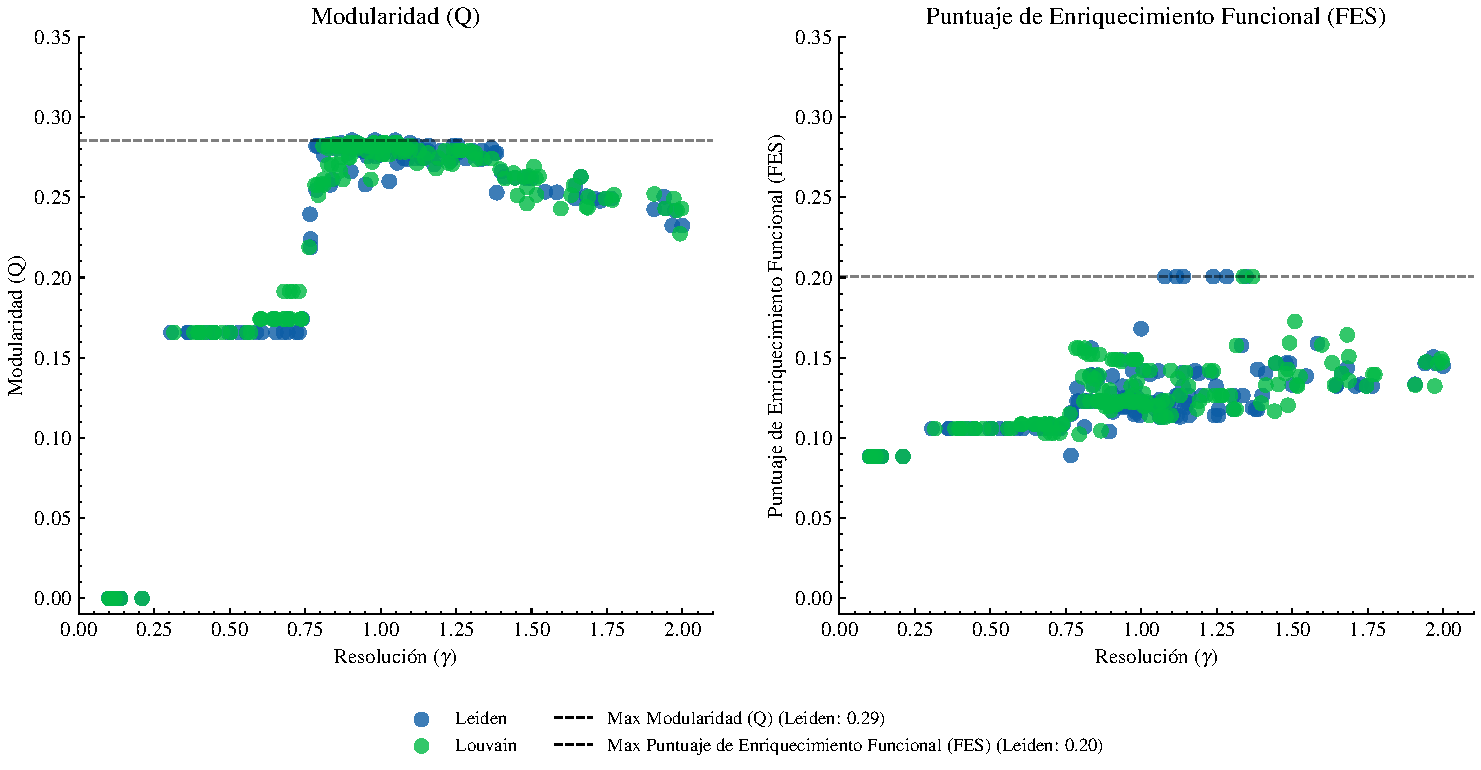
\includegraphics[width=.96\textwidth]{../results/plots/optimization/hyperparameter_vs_metric.pdf}
	\caption{Valores de resolución (\(\gamma\)) explorados por algoritmo, frente al rendimiento evaluado sobre el clustering obtenido. Leiden obtiene por un margen considerable la mejor modularidad, mientras que Louvain obtiene el mejor valor del FES por una diferencia despreciable.}
	\label{fig:slice_plot}
\end{figure}


\subsection{Clustering}

\begin{figure}[htbp]
	\centering
	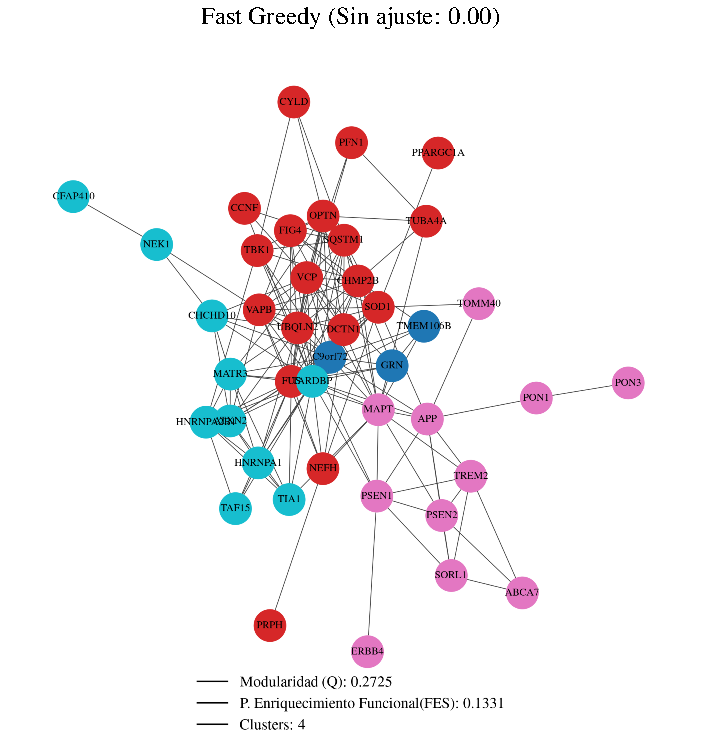
\includegraphics[width=.75\textwidth]{../results/plots/clustering/fast greedy_clustering.pdf}
	\caption{Resultados de clustering para el algoritmo Fast-Greedy. Este clustering será considerado como nuestra base. No se ha ajustado ningún hiperparámetro para este método.}
	\label{fig:fastgreedy_clustering}
\end{figure}

\begin{figure}[htbp]
	\centering
	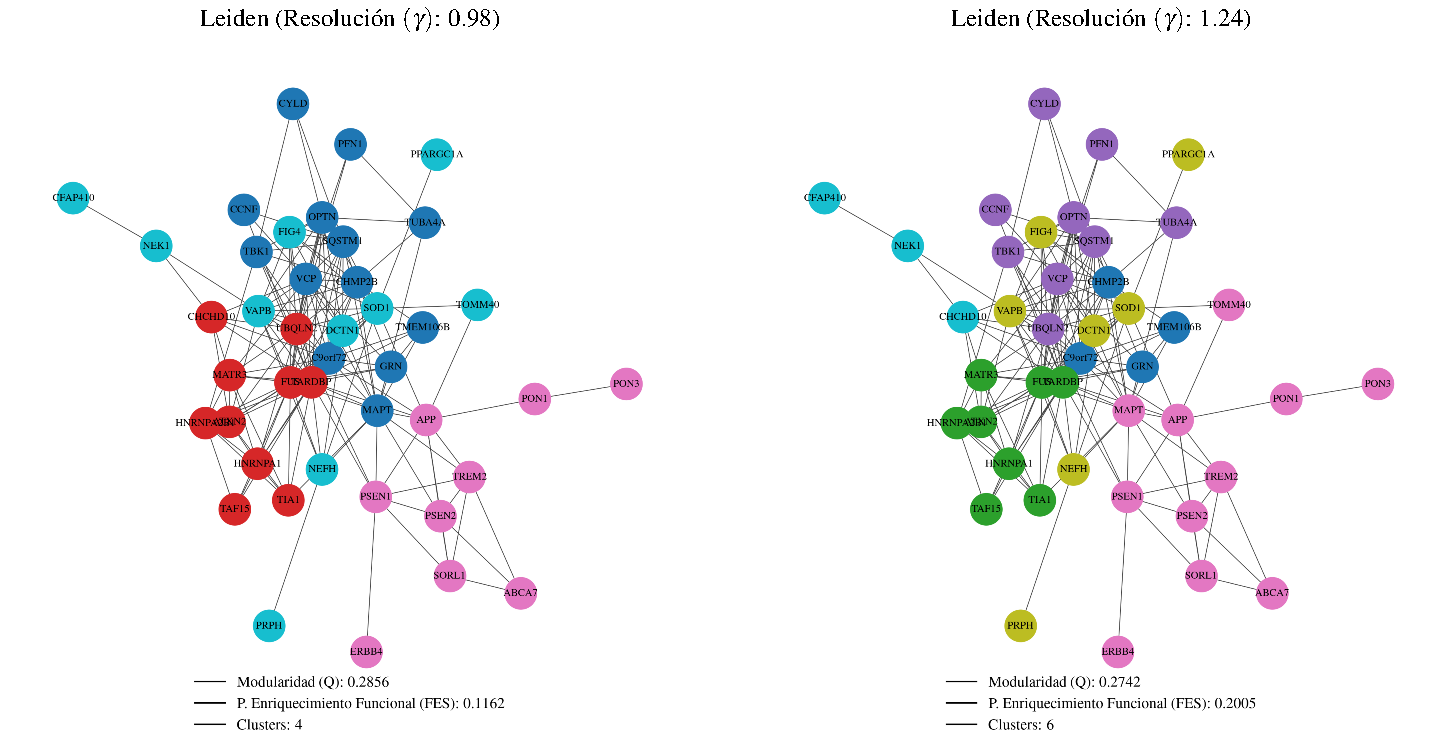
\includegraphics[width=.96\textwidth]{../results/plots/clustering/leiden_clustering.pdf}
	\caption{Resultados de clustering para el algoritmo Leiden. Se presentan dos resultados, que corresponden a las soluciones Pareto-óptimas extremas (\(max(Q)\) ó \(max(FES)\)).}
	\label{fig:leiden_clustering}
\end{figure}

\begin{figure}[htbp]
	\centering
	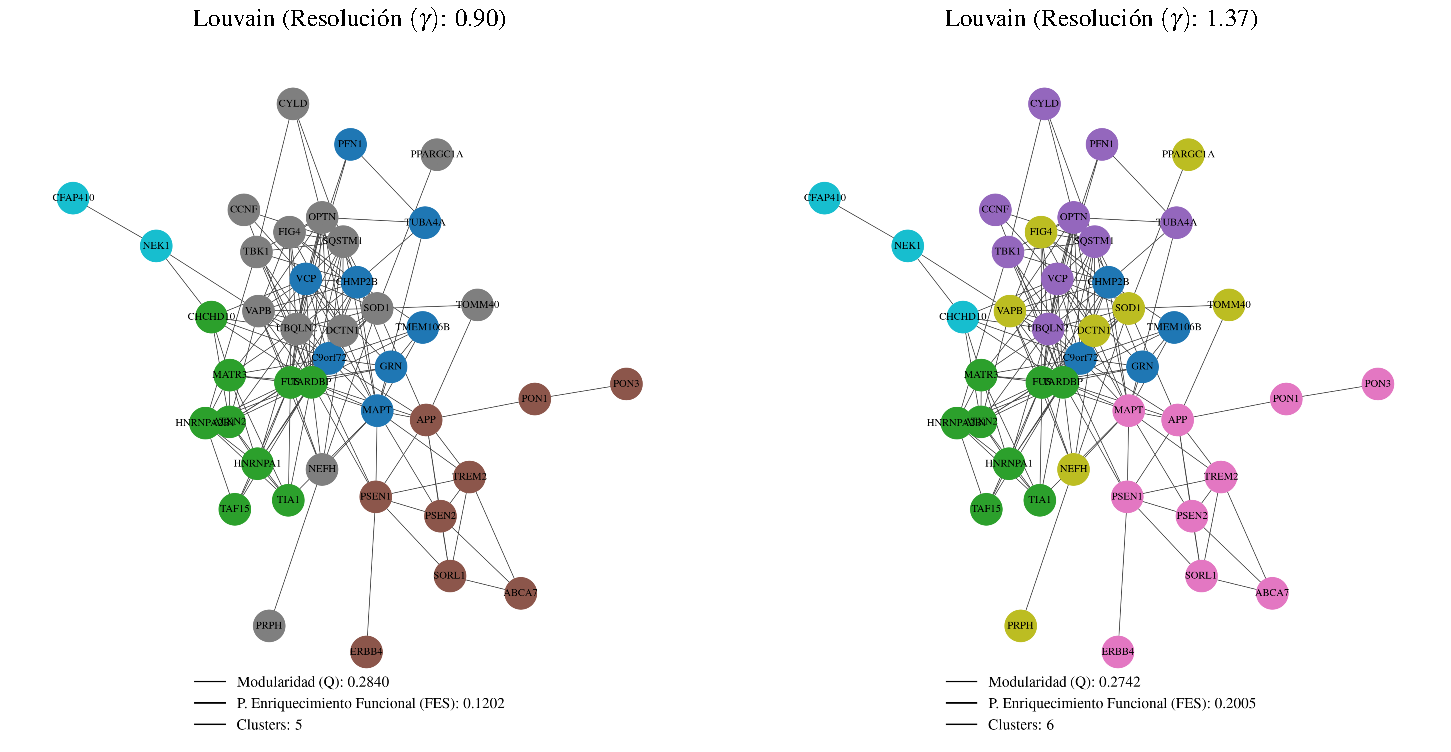
\includegraphics[width=.96\textwidth]{../results/plots/clustering/louvain_clustering.pdf}
	\caption{Resultados de clustering para el algoritmo Louvain. Se presentan dos resultados, que corresponden a las soluciones Pareto-óptimas extremas (\(max(Q)\) ó \(max(FES)\)).}
	\label{fig:louvain_clustering}
\end{figure}

\subsection{Análisis Funcional}